\documentclass[14pt]{extbook}
\usepackage{multicol, enumerate, enumitem, hyperref, color, soul, setspace, parskip, fancyhdr} %General Packages
\usepackage{amssymb, amsthm, amsmath, bbm, latexsym, units, mathtools} %Math Packages
\everymath{\displaystyle} %All math in Display Style
% Packages with additional options
\usepackage[headsep=0.5cm,headheight=12pt, left=1 in,right= 1 in,top= 1 in,bottom= 1 in]{geometry}
\usepackage[usenames,dvipsnames]{xcolor}
\usepackage{dashrule}  % Package to use the command below to create lines between items
\newcommand{\litem}[1]{\item#1\hspace*{-1cm}\rule{\textwidth}{0.4pt}}
\pagestyle{fancy}
\lhead{Module7}
\chead{}
\rhead{Version C}
\lfoot{4758-2646}
\cfoot{}
\rfoot{testing}
\begin{document}

\begin{enumerate}
\litem{
Determine the domain of the function below.\[ f(x) = \frac{4}{15x^{2} -13 x -20} \]\begin{enumerate}[label=\Alph*.]
\item \( \text{All Real numbers except } x = a, \text{ where } a \in [-20, -19] \)
\item \( \text{All Real numbers except } x = a \text{ and } x = b, \text{ where } a \in [-20, -19] \text{ and } b \in [15, 16] \)
\item \( \text{All Real numbers except } x = a \text{ and } x = b, \text{ where } a \in [-1.8, 1.2] \text{ and } b \in [-0.33, 4.67] \)
\item \( \text{All Real numbers.} \)
\item \( \text{All Real numbers except } x = a, \text{ where } a \in [-1.8, 1.2] \)

\end{enumerate} }
\litem{
Determine the domain of the function below.\[ f(x) = \frac{6}{12x^{2} +21 x + 9} \]\begin{enumerate}[label=\Alph*.]
\item \( \text{All Real numbers except } x = a \text{ and } x = b, \text{ where } a \in [-12.57, -11.6] \text{ and } b \in [-9.5, -8.48] \)
\item \( \text{All Real numbers except } x = a, \text{ where } a \in [-12.57, -11.6] \)
\item \( \text{All Real numbers except } x = a \text{ and } x = b, \text{ where } a \in [-1.37, -0.85] \text{ and } b \in [-0.94, -0.33] \)
\item \( \text{All Real numbers except } x = a, \text{ where } a \in [-1.37, -0.85] \)
\item \( \text{All Real numbers.} \)

\end{enumerate} }
\litem{
Solve the rational equation below. Then, choose the interval(s) that the solution(s) belongs to.\[ \frac{-3x}{5x -7} + \frac{-2x^{2}}{-15x^{2} +6 x + 21} = \frac{-6}{-3x -3} \]\begin{enumerate}[label=\Alph*.]
\item \( x \in [-7.5,-4.5] \)
\item \( x_1 \in [0.92, 6.92] \text{ and } x_2 \in [-7.5,-2.5] \)
\item \( x \in [-4,0] \)
\item \( \text{All solutions lead to invalid or complex values in the equation.} \)
\item \( x_1 \in [0.92, 6.92] \text{ and } x_2 \in [-3.6,7.4] \)

\end{enumerate} }
\litem{
Choose the graph of the equation below.\[ f(x) = \frac{1}{(x + 1)^2} + 2 \]\begin{enumerate}[label=\Alph*.]
\begin{multicols}{2}\item 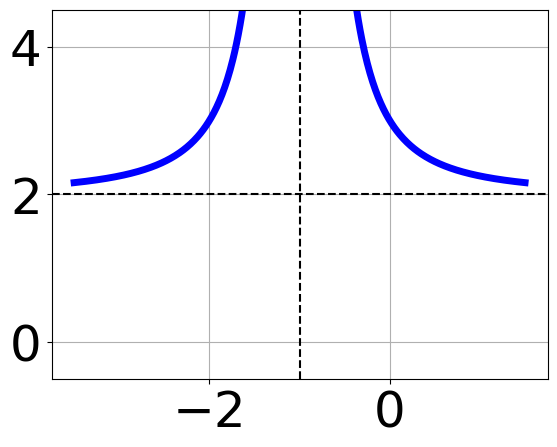
\includegraphics[width = 0.3\textwidth]{../Figures/rationalEquationToGraphAC.png}\item 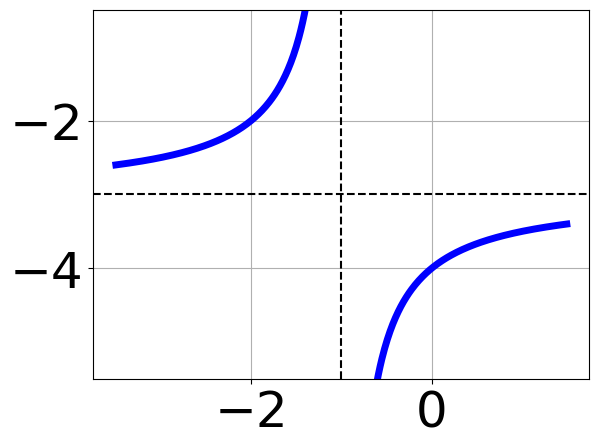
\includegraphics[width = 0.3\textwidth]{../Figures/rationalEquationToGraphBC.png}\item 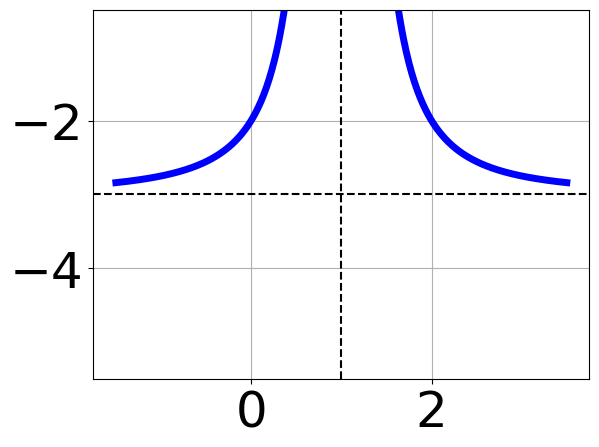
\includegraphics[width = 0.3\textwidth]{../Figures/rationalEquationToGraphCC.png}\item 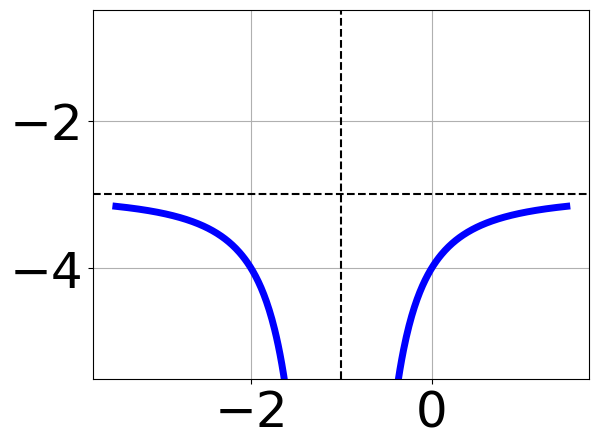
\includegraphics[width = 0.3\textwidth]{../Figures/rationalEquationToGraphDC.png}\end{multicols}\item None of the above.
\end{enumerate} }
\litem{
Choose the graph of the equation below.\[ f(x) = \frac{1}{(x + 1)^2} + 1 \]\begin{enumerate}[label=\Alph*.]
\begin{multicols}{2}\item 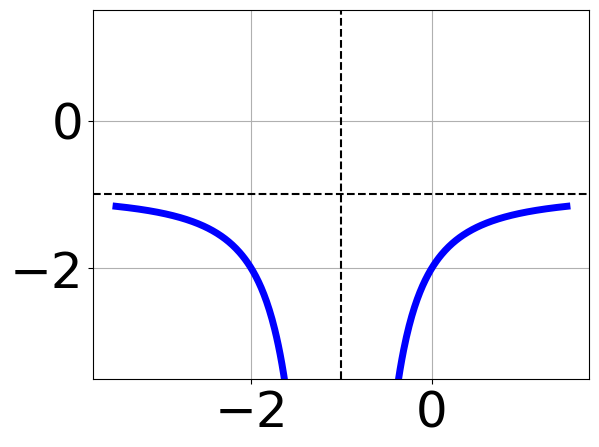
\includegraphics[width = 0.3\textwidth]{../Figures/rationalEquationToGraphCopyAC.png}\item 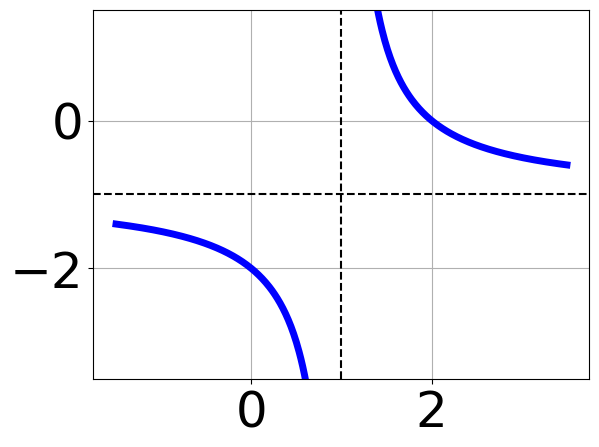
\includegraphics[width = 0.3\textwidth]{../Figures/rationalEquationToGraphCopyBC.png}\item 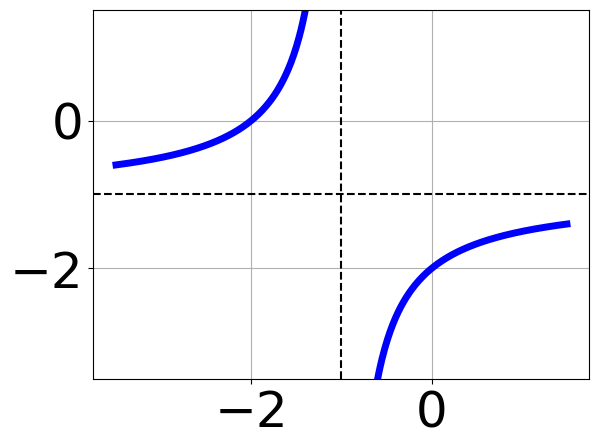
\includegraphics[width = 0.3\textwidth]{../Figures/rationalEquationToGraphCopyCC.png}\item 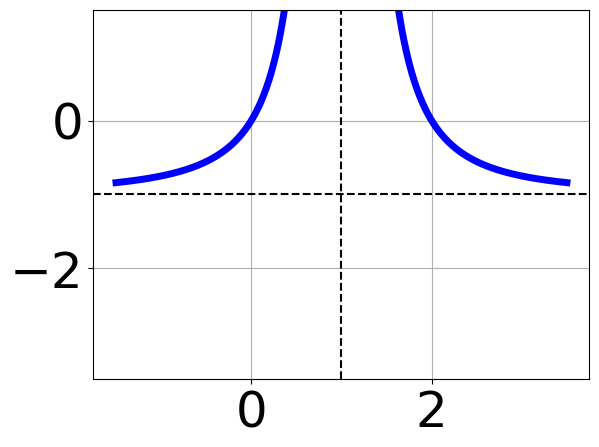
\includegraphics[width = 0.3\textwidth]{../Figures/rationalEquationToGraphCopyDC.png}\end{multicols}\item None of the above.
\end{enumerate} }
\litem{
Choose the equation of the function graphed below.
\begin{center}
    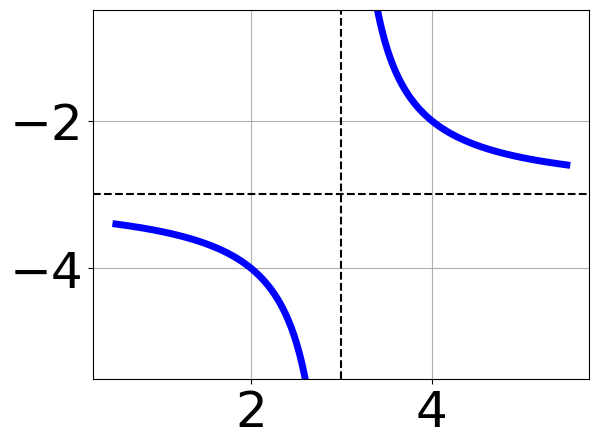
\includegraphics[width=0.5\textwidth]{../Figures/rationalGraphToEquationCopyC.png}
\end{center}
\begin{enumerate}[label=\Alph*.]
\item \( f(x) = \frac{-1}{(x - 2)^2} + 3 \)
\item \( f(x) = \frac{-1}{x - 2} + 3 \)
\item \( f(x) = \frac{1}{x + 2} + 3 \)
\item \( f(x) = \frac{1}{(x + 2)^2} + 3 \)
\item \( \text{None of the above} \)

\end{enumerate} }
\litem{
Solve the rational equation below. Then, choose the interval(s) that the solution(s) belongs to.\[ \frac{56}{-48x + 24} + 1 = \frac{56}{-48x + 24} \]\begin{enumerate}[label=\Alph*.]
\item \( x_1 \in [-1.5, -0.2] \text{ and } x_2 \in [0.5,3.5] \)
\item \( x_1 \in [-0.1, 1.7] \text{ and } x_2 \in [0.5,3.5] \)
\item \( \text{All solutions lead to invalid or complex values in the equation.} \)
\item \( x \in [-0.5,1.5] \)
\item \( x \in [-1.5,-0.2] \)

\end{enumerate} }
\litem{
Solve the rational equation below. Then, choose the interval(s) that the solution(s) belongs to.\[ \frac{12}{-12x -48} + 1 = \frac{12}{-12x -48} \]\begin{enumerate}[label=\Alph*.]
\item \( x \in [-4.0,-3.0] \)
\item \( x \in [3,5] \)
\item \( \text{All solutions lead to invalid or complex values in the equation.} \)
\item \( x_1 \in [-4, -2] \text{ and } x_2 \in [3,7] \)
\item \( x_1 \in [-4, -2] \text{ and } x_2 \in [-4,-3] \)

\end{enumerate} }
\litem{
Solve the rational equation below. Then, choose the interval(s) that the solution(s) belongs to.\[ \frac{-6x}{-6x + 7} + \frac{-6x^{2}}{-24x^{2} -8 x + 42} = \frac{-7}{4x + 6} \]\begin{enumerate}[label=\Alph*.]
\item \( x_1 \in [-0.63, 0.68] \text{ and } x_2 \in [-8.12,0.88] \)
\item \( \text{All solutions lead to invalid or complex values in the equation.} \)
\item \( x \in [-4.2,-2.6] \)
\item \( x \in [-2.06,-1.19] \)
\item \( x_1 \in [-0.63, 0.68] \text{ and } x_2 \in [-2.83,8.17] \)

\end{enumerate} }
\litem{
Choose the equation of the function graphed below.
\begin{center}
    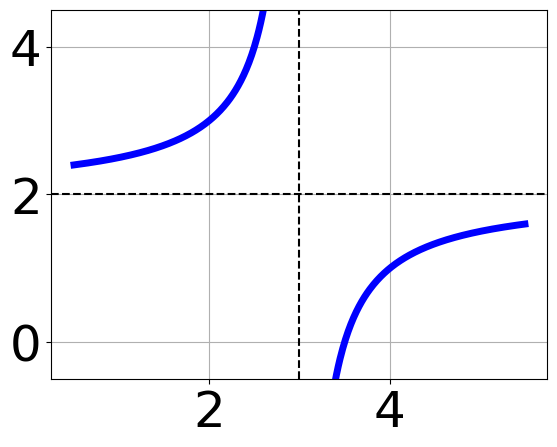
\includegraphics[width=0.5\textwidth]{../Figures/rationalGraphToEquationC.png}
\end{center}
\begin{enumerate}[label=\Alph*.]
\item \( f(x) = \frac{1}{(x + 2)^2} + 1 \)
\item \( f(x) = \frac{1}{x + 2} + 1 \)
\item \( f(x) = \frac{-1}{x - 2} + 1 \)
\item \( f(x) = \frac{-1}{(x - 2)^2} + 1 \)
\item \( \text{None of the above} \)

\end{enumerate} }
\end{enumerate}

\end{document}